\chapter{Proof of concept, praktische Anwendung}\label{chap:experiments}
Die lokale Auswertung persönlicher Daten ist das Hauptargument für eine dezentralisierte Smart Home Steuerung aus Sicht von Konsumenten, die, wie in der Befragung des IDC einsehbar \cite{IDC}, häufig angeben, dass die mögliche Auswertung ihrer Informationen durch Dritte ein ausschlaggebender Faktor gegen die Anschaffung eines solchen Systems darstellt. 
Der Aufbau dieser Anwendung sieht daher vor, die Datenanalyse vollständig innerhalb des Heimnetzes des Anwenders durchzuführen, sich also auf eine „Small Data“ Analyse zu beschränken und so den Einwänden, die mit „Big Data Mining“ einhergehen, vorzugreifen. 

Um den theoretisch skizzierten Anwendungsfall praktisch zu untersuchen, wird der gewählte Process Mining Algorithmus auf einem einfachen, im lokalen Netz erreichbaren, Server als Dienst implementiert. Dieser wartet auf das Eintreffen von Eventlogs aus einem Smart Home, verarbeitet die Rohdaten und leitet das resultierende Modell an eine mobile Anwendung weiter. Die Anwendung soll dem Bewohner die Möglichkeit geben, die vom Process Mining Algorithmus extrahierten Regeln im Smart Home zu integrieren. Wird die Regel vom Bewohner akzeptiert, übernimmt der lokale Server die Automatisierung der Abläufe auf den relevanten vernetzten Geräten.

\section{Aufbau und Komponenten der praktischen Anwendung}
Das Smart Home Modell, das zu Testzwecken in dieser Arbeit dient, wird vom ITOM Institut der FH Aachen betrieben und ist mit unterschiedlichen Sensoren und Aktoren ausgestattet. 
Außerdem wird die Android Anwendung „Grafischer Regeleditor“, die zuvor im Rahmen einer Abschlussarbeit am ITOM Institut entstandenen ist, als Grundlage für die Kommunikation mit dem Anwender genutzt und um die Funktion der automatisierten Regelerkennung erweitert. 
Die Funktionalität der Kommunikation mit einem lokalen Server und das manuelle Anlegen von Regeln für IoT Geräte ist bereits in der Anwendung integriert.

Die Auswertung durch das Process Mining, die Archivierung der Eventlogs und die Kommunikation mit den vernetzten Geräten des Smart Homes werden von einem einfachen Server mit ARM-Prozessor übernommen, konkret handelt es sich dabei um ein Raspberry Pi 3.0. Um den Anwender über neue erkannte Muster zu informieren, wird jeweils eine Benachrichtigung an das Mobiltelefon versandt. Das Versenden der Benachrichtigung übernimmt der \textit{firebase}\footnote{https://firebase.google.com/} Dienst. Diese Aufgabe könnte, um den Aspekt des Datenschutzes voll zu erfüllen, ebenfalls von einem lokalen Dienst durchgeführt werden.

\section{Dienste und Skripte auf dem Heimserver}
Da die Anwendung auf der Architektur des Projekts „Grafischer Regeleditor“ aufbaut, wird in dieser Arbeit vorausgesetzt, dass openHab als Dienst im Heimnetzwerk des Anwenders eingerichtet ist. Dieser Dienst ist eine essentielle Komponente der Anwendung, er ist verantwortlich für die Kommunikation mit den IoT Geräten. Sowohl die Erzeugung der Protokolldatei als auch die Ausführung von Regeln erfolgt mithilfe von openHab. 

Die quelloffene openHAB (open Home Automation Bus) Automatisierungssoftware implementiert eine weite Bandbreite herstellerabhängiger Standards und gewährleistet so die Kommunikation zwischen unterschiedlichen vernetzten Geräten. Die Automatisierungslogik der openHAB-Software ist als einfacher Regex-Agent anzusehen. 
Um die Brücke von der unverarbeiteten gesammelten Menge an Ereigniseinträgen zu einer neuen, automatisiert erkannten Regel zu schlagen wird ein Skript auf dem Server hinterlegt, welches periodisch alle notwendigen Verarbeitungsschritte des Prozesses aufruft. In regelmäßigen Abständen wird das auf dem lokalen Server hinterlegte Eventlog geladen und zunächst vom CSV in das XES Format konvertiert. 

Diese Konvertierung ist ein simpler Vorgang, bei dem jeder Eintrag, der in der CSV Datei eine einzelne Instanz einer Aktion eines IoT Geräts repräsentiert, in seine Komponenten teilt und in das XES Format übertragen wird. Die Komponenten umfassen, wie in Abschnitt \ref{sec:xes} beschrieben, den Zeitstempel, den Namen des Geräts - in der Form in der er unter openHab hinterlegt ist - sowie die Aktion oder den Sensorwert der den Eintrag erzeugt hat. Die einzelnen Komponenten werden im Ausgangsformat von XML-Tags eingeschlossen. Dieser Schritt ermöglicht die Verarbeitung der Daten mit ProM.

%Bei der Untersuchung von unverarbeiteten Eventlogs, die im Smart Living Modellhaus des ITOM Institus entstanden sind, ist erkennbar, dass es bei einigen der im Haus integrierten Geräte dazu kommt, dass sie ein Zeitstempelformat nutzen, welches die Sekunden nicht angibt. Hier ist also vor der Konvertierung ein Vorverarbeitungssschritt notwendig, der über jede Zeile iteriert und die Stempel einander angleicht. Da kein universeller Standard für IoT Logs Branchenweit akzeptiert wird und die Hersteller diese beliebig formatieren können, sind mit jedem weiteren angeschlossenen Gerät auch weitere Abweichungen von der erwarteten Form nicht auszuschließen. Um diesem Problem entgegenzuwirken können Tools wie ‚syslog-ng‘ eingesetzt werden, die in der Lage sind die meisten Formen von Eventlogs auf ein einheitliches Format zu bringen.

Im nächsten Schritt ruft das Skript ein in der Programmiersprache Java geschriebenes Programm auf, welches Process Mining auf dem neu entstandenen XES Dokument durchführt. Konkret wird dafür ProM auf dem Server gestartet und das Heuristic Miner Plugin ausgewählt.
Über Parameter kann die Analyse durch das Heuristic Miner Plugin zusätzlich angepasst werden, etwa um Rauschdaten zu unterdrücken oder weitere Attribute bei der Datenanalyse zu berücksichtigen, falls diese im Eventlog gegeben sind. Der Vorverarbeitungsschritt der Rauschreduzierung ist unerlässlich für die Regelfindung. Es sollten keine Knoten als Teil des Regelvorschlags an den Nutzer gelangen, die nicht auch Teil seines regulären Ablaufs sind. 


In dieser Arbeit wird der Schwellwert für Rauschdaten über einen iterativen Prozess gesucht. Da es im Vorfeld keine Information über die Menge der Rauschdaten im zu untersuchenden Eventlog geben kann, wird wie folgt verfahren. 

\begin{figure}[!h]
    \centering
    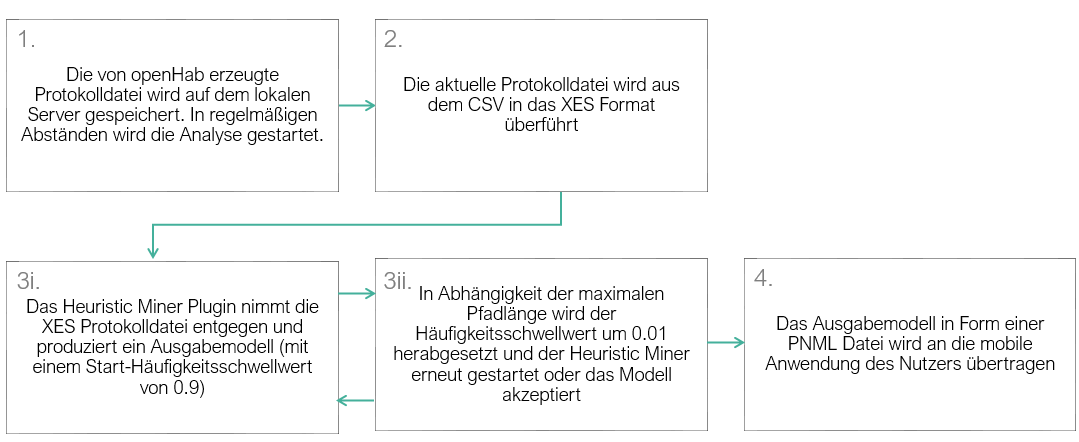
\includegraphics[width=\textwidth,origin=c]{figures/Appbildungen/ServerSchritte.PNG}
    \caption{Verarbeitungsschritte zur Auswertung der Smart Home Daten auf dem Server}
    \label{fig:server}
\end{figure}

\newpage
Ziel ist es ein Modell der häufigsten, kurzen Routinen zu finden. Genauer soll eine Regel mindestens eine Vorbedingung und eine Aktion enthalten, maximal drei Vorbedingungen werden akzeptiert. Nachdem ein Modell aus zwei Knoten gefunden wurde, wird dieses um einen weiteren Knoten erweitert, wenn die Auftrittshäufigkeit des Elements mindestens so hoch ist wie die bisherigen Elemente. Der Regler für den Häufigkeitsschwellwert (im Plugin 'frequency' genannt) wird mit einem Startwert von 0.9 initialisiert, ein Petri Netz erzeugt und dessen Knoten gezählt. Der Schwellwert wird inkrementell (Schritte von 0.1) verringert, bis eine Veränderung im Ausgabemodell auftritt. Ist die Auftrittshäufigkeit des neuen Elements im Ausgabemodell im Vergleich zum Vorangegangen geringer, wird das Vorgängermodell als korrekte Regel akzeptiert. Liegt die Auftrittshäufigkeit auf dem selben Niveau, wird der Wert weiter dekrementiert, bis sich das Modell verändert. Tritt ein weiterer Eintrag im Ausgabemodell auf, wird wieder die Auftrittshäufigkeit verglichen. Dieser Vorgang wird wiederholt, bis maximal drei Vorbedingungen eine Regel bilden oder die Auftrittshäufigkeit des neuen Eintrags unter dem der anderen Einträge liegt.

Ist dieser Prozess abgeschlossen, ist eine Regel gefunden worden.
Das Modell des Miners wird zunächst im PNML Format gespeichert, welches Petri Netze nach dem XML Schema beschreibt. Das Petri Netz wird dann in ein If This Then That Schema überführt.

Abschließend enthält das Skript einen Aufruf an ein kurzes, in Python geschriebenen Programmm, welches den Firebase Dienst dazu auffordert eine Benachrichtigung an das mobile Gerät des Anwenders zu senden, welche den Inhalt des neuen Dokuments übermittelt. Der Prozess, der auf dem Server stattfindet, ist in wenigen Schritten auf Abbildung  \ref{fig:server} dargestellt.

\section{Mobile Anwendung als Steuerungs- und Kommunikationsschnittstelle}

Um die Regeleditor Anwendung um die Kommunikation mit einem dedizierten Firebase Dienst zu erweitern, wird eine Klasse PMFireBaseMessagingService angelegt. Diese ist dafür verantwortlich, die Regel entgegenzunehmen und übergibt sie an die im Rahmen dieser Arbeit erzeugte \textit{PMRule} Klasse, die verantwortlich für die Überführung der empfangenen Nachricht in eine Regelform ist. Konkret wird dies von der Funktion parseReceivedRule() übernommen.
\small
\begin{lstlisting}[language=Java]
       private void parseReceivedRule(JSONArray ruleJSON) throws JSONException {
        PMRule r = new PMRule();
        int lastEntry = 0 ;
        for(int j=0;j<ruleJSON.length();j++){
            Log.d("processmining", "rules Array"+j+": "+ruleJSON.getJSONArray(j));

            if(ruleJSON.getJSONArray(j).length()>1){
                lastEntry = ruleJSON.getJSONArray(j).length()-1;
                Vector<String> preconditions = new Vector<>();
                for(int i=lastEntry; i>=0;i--){
                    if(i==lastEntry)
                        r.setAction(ruleJSON.getJSONArray(j).getString(i));
                    else
                        preconditions.add(ruleJSON.getJSONArray(j).getString(i));
                }
                r.setPrecondition(preconditions);
                PMRules.add(r);
                Log.d("processmining", "IF: "+r.getPrecondition()+" THEN: "+r.getAction());
            }
        }
        Intent pmIntent = new Intent(Main.this, ProcessMiningRuleActivity.class);
        pmIntent.putExtra("IF", r.getPrecondition());
        pmIntent.putExtra("THEN", r.getAction());
        startActivity(pmIntent);
    }
\end{lstlisting}

\begin{wrapfigure}{R}{0.5\textwidth}
  \begin{center}
    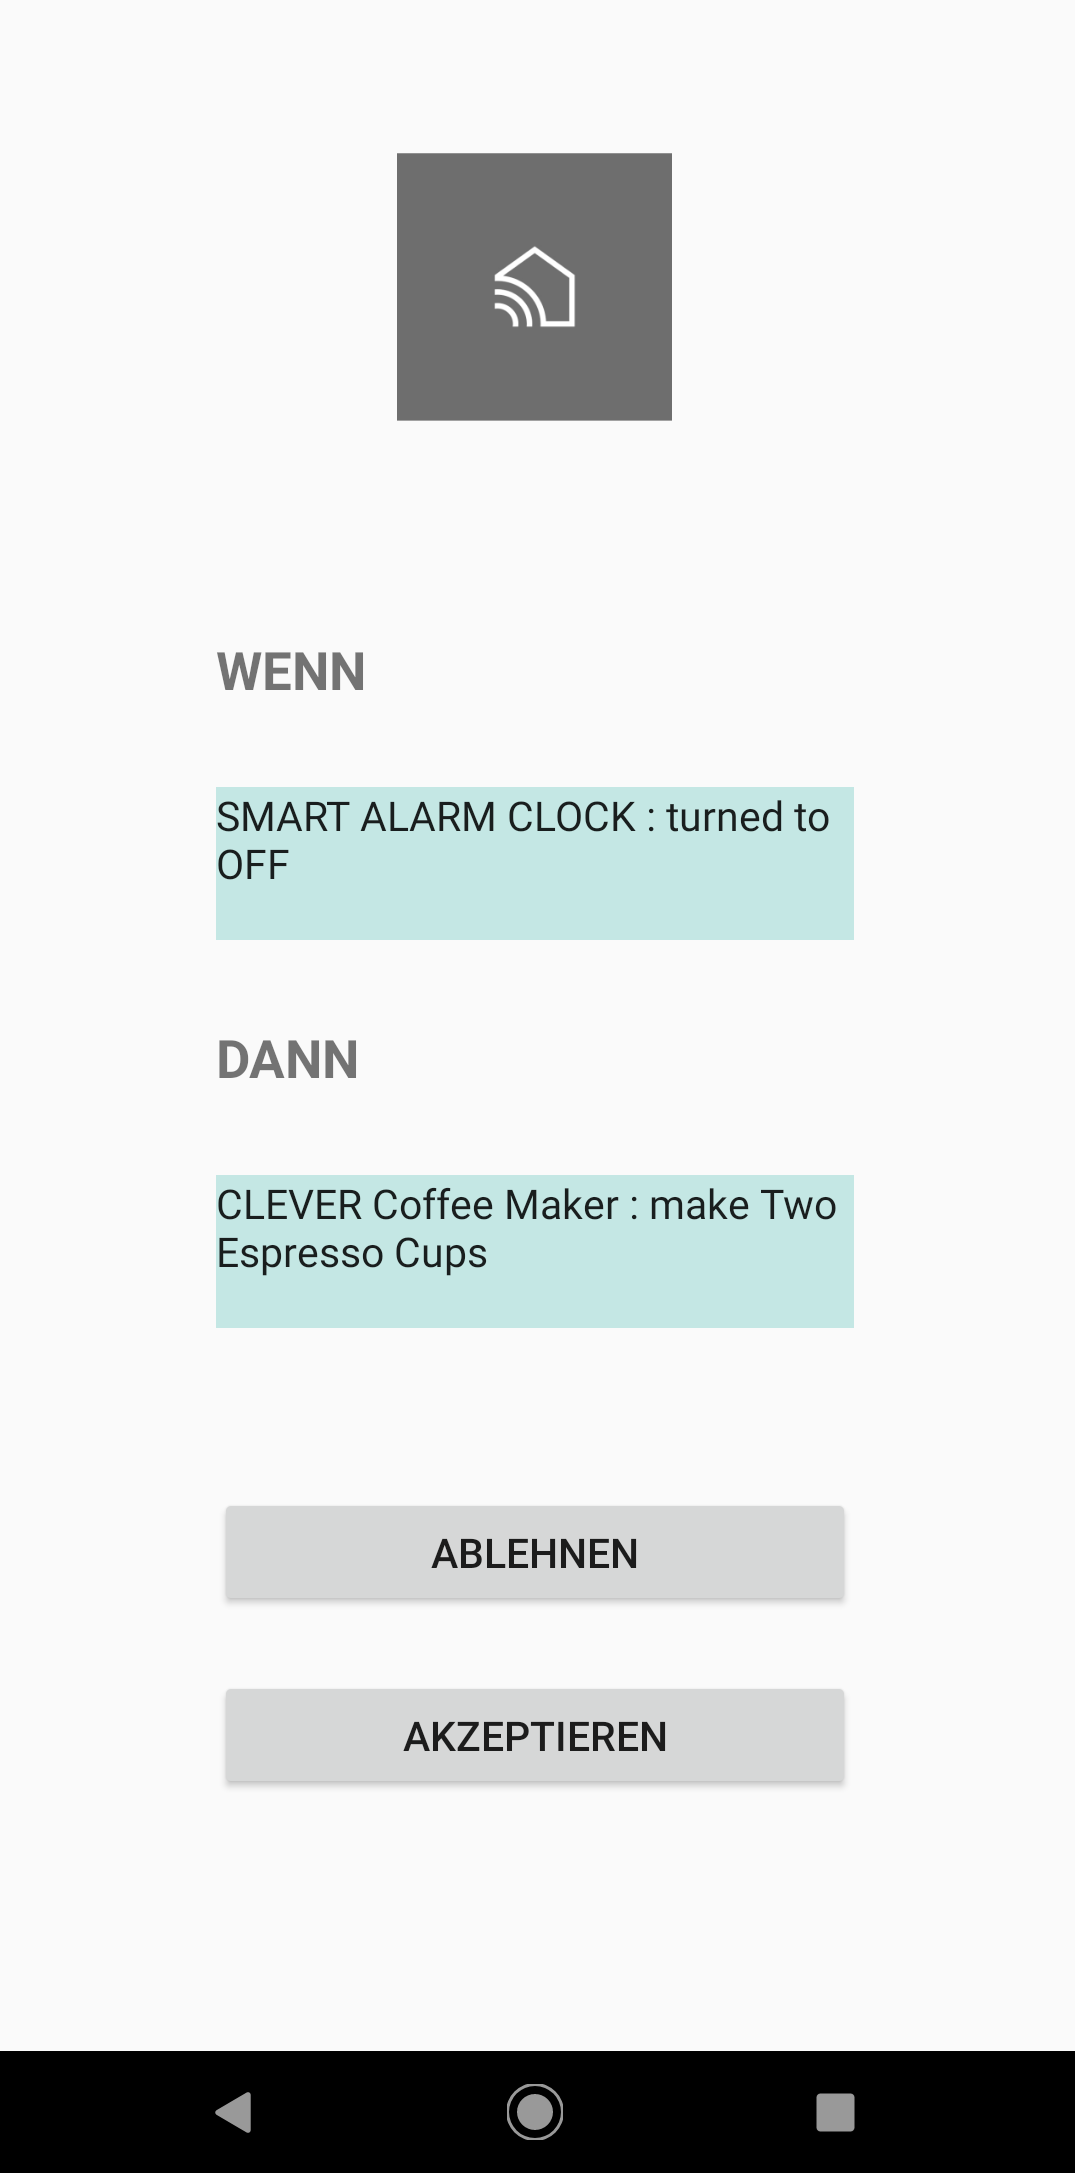
\includegraphics[width=0.3\textwidth]{figures/Appbildungen/newRuleDialog.png}
  \end{center}
  
  \caption{Proof of Concept: Dialog bei Eingang neuer erkannter Regel}\label{fig:dialog}
\end{wrapfigure}
\normalsize

Diese Funktion erlaubt das klassifizieren der Elemente in Vor- und Nachbedingungen, die dann direkt in die vorhandene Datenbank der Anwendung "Grafischer Regeleditor" eingefügt werden können.

Durch die Benachrichtigung, die auf dem Mobilen Gerät angezeigt wird, wenn der Firebase Dienst eine neue Regel zugestellt hat, wird ein Dialog innerhalb der „Grafischer Regeleditor“ Anwendung gestartet. Ein Beispiel für den Dialog ist auf Abbildung \ref{fig:dialog} zu sehen. Die Vorbedingungen und Aktionen der Regel werden im Wenn – Dann Format dargestellt. Der Nutzer hat zunächst die Möglichkeit die Regel zu akzeptieren oder abzulehnen. Wird sie abgelehnt, wird die Regel nicht ins lokale openHab System aufgenommen und eine entsprechende Feedback Nachricht an den Server übermittelt. Dieser Schritt soll verhindern, dass eine vom Anwender nicht erwünschte Regel wiederholt vorgeschlagen wird. Der Server soll neue Regeln zunächst gegen bestehende und abgelehnte Regeln abgleichen, bevor eine neue Anfrage an den Benutzer gestellt wird.

Wird der Vorschlag vom Anwender akzeptiert, wird er zu einem weiteren Fenster weitergeleitet, welches ihm die Option bietet, die Regel ohne Anpassungen zu übernehmen, oder aber die vorgeschlagene Regel zu editieren. Beispielsweise können weitere Vorbedingungen oder Aktionen hinzugefügt oder entfernt werden. 


Für diese Funktionalität wird auf das Regelwerk der zur Verfügung gestellten „Grafischer Regeleditor“ App zurückgegriffen. 

Nachdem die Regel vom Nutzer akzeptiert worden ist, wird sie wie in der Vorgängerversion der Anwendung auch in eine SQLite Datenbank eingetragen. OpenHab empfängt die aktualisierten Regeln aus der Datenbannk und wird nun die Aktion ausführen, sobald die vermerkten Vorbedingungen erfüllt sind.
Weitere Funktionen wie das nachträgliche Entfernen oder Editieren der Regeln stehen dem Anwender wie bereits in der Vorgängerversion zur Verfügung.
Der clientseitige Prozess wird in Abbildung \ref{fig:Kommunikationsablauf} noch einmal im BPMN Format graphisch dargestellt.
\newpage
\begin{figure}[!ht]
    \centering
    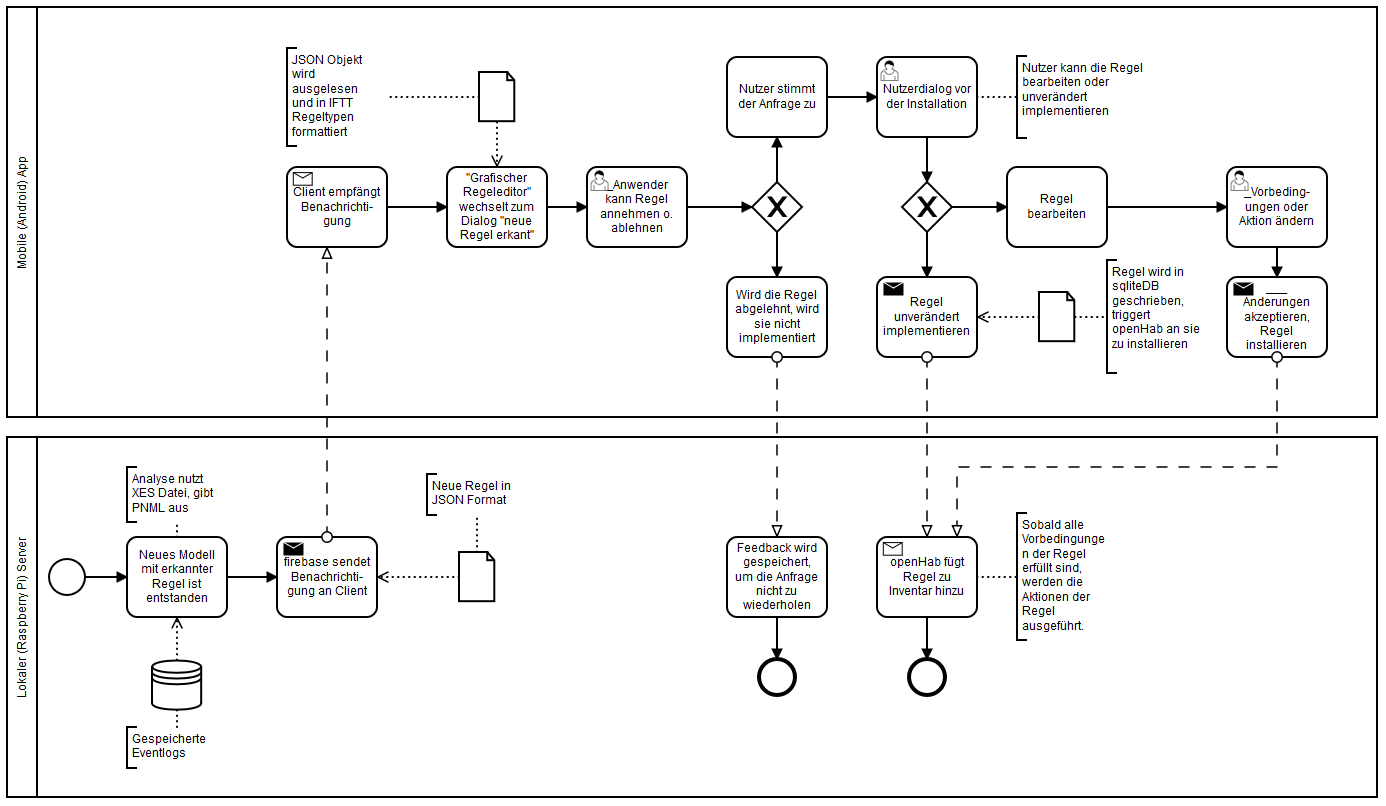
\includegraphics[width= 1.47\textwidth, angle=90,origin=c]{figures/Appbildungen/diagramm_app.PNG}
    \caption{Ablauf der Kommunikation zwischen Endanwender und lokalem Server}
    \label{fig:Kommunikationsablauf}
\end{figure}